% Created 2020-07-06 lun 12:34
% Intended LaTeX compiler: pdflatex
\documentclass[presentation,aspectratio=169]{beamer}
\usepackage[utf8]{inputenc}
\usepackage[T1]{fontenc}
\usepackage{graphicx}
\usepackage{grffile}
\usepackage{longtable}
\usepackage{wrapfig}
\usepackage{rotating}
\usepackage[normalem]{ulem}
\usepackage{amsmath}
\usepackage{textcomp}
\usepackage{amssymb}
\usepackage{capt-of}
\usepackage{hyperref}
\usepackage{khpreamble}
\usepackage{amssymb}
\usepackage{tcolorbox}
\DeclareMathOperator{\shift}{q}
\DeclareMathOperator{\diff}{p}
\usetheme{default}
\author{Kjartan Halvorsen}
\date{2020-07-06}
\title{Control Computarizado - Estabilidad de sistemas discretas}
\hypersetup{
 pdfauthor={Kjartan Halvorsen},
 pdftitle={Control Computarizado - Estabilidad de sistemas discretas},
 pdfkeywords={},
 pdfsubject={},
 pdfcreator={Emacs 26.3 (Org mode 9.3.6)}, 
 pdflang={English}}
\begin{document}

\maketitle

\section{Intro}
\label{sec:orgcc8a22a}
\begin{frame}[label={sec:org02967ac}]{Repetición: Controlador discreto para el brazo del disco duro}
Usando \(J=1\) y  \(h=1\).
\begin{center}
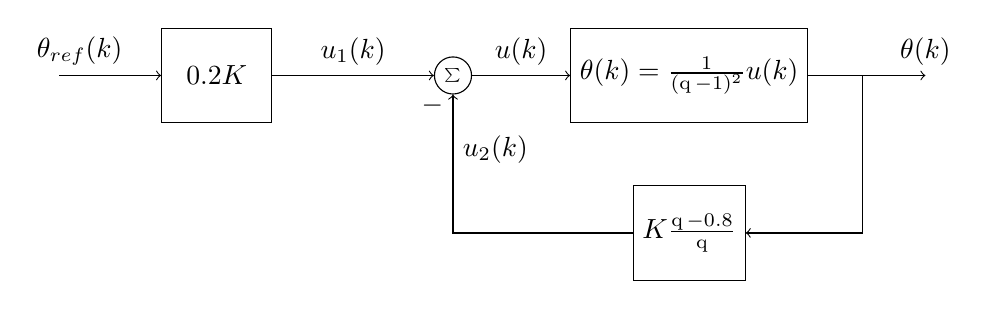
\begin{tikzpicture}
\tikzset{node distance=2cm, 
    block/.style={rectangle, draw, minimum height=12mm, minimum width=14mm},
    sumnode/.style={circle, draw, inner sep=2pt}        
}

  \node[coordinate] (input) {};
  \node[block, right of=input] (TR) {$0.2K$};
  \node[sumnode, right of=TR, node distance=30mm] (sum) {\tiny $\sum$};
  \node[block,right of=sum, node distance=30mm] (plant) {$\theta(k) = \frac{1}{(\shift-1)^2}u(k)$};
  %\node[sumnode, right of=plant, node distance=30mm] (sumdist) {$\sum$};
  %\node[coordinate, above of=sumdist, node distance=15mm] (dist) {};
  %\node[coordinate, right of=sumdist, node distance=15mm] (measure) {};
  \node[coordinate, right of=plant, node distance=30mm] (output) {};
  \node[coordinate, right of=plant, node distance=22mm] (measure) {};
  %\node[sumnode,below of=measure, node distance=25mm] (sumnoise) {$\sum$};
  %\node[coordinate, right of=sumnoise, node distance=15mm] (noise) {};
  \node[block,below of=plant, node distance=20mm] (SR) {$K\frac{\shift - 0.8}{\shift}$};
  \draw[->] (input) -- node[above, pos=0.2] {$\theta_{ref}(k)$} (TR);
  \draw[->] (TR) -- node[above] {$u_1(k)$} (sum);
  \draw[->] (sum) -- node[above] {$u(k)$} (plant);
  \draw[->] (plant) -- node[at end, above] {$\theta(k)$} (output);
  \draw[->] (measure) |- (SR);
  \draw[->] (SR) -| (sum) node[right, pos=0.8] {$u_2(k)$} node[left, pos=0.96] {$-$};
\end{tikzpicture}
\end{center}
Ecuación en diferencias para el sistema de lazo cerrado:
\[ \theta(k+3) -2\theta(k+2) + (1+K)\theta(k+1) - 0.8K\theta(k) = 0.2K\theta_{ref}(k+1)\]
Ecuación característica:
\[ \alpha^3 - 2\alpha^2 + (1+K)\alpha - 0.8K = 0\]
\end{frame}

\begin{frame}[label={sec:org41f2b6c}]{Repetición: Controlador discreto para el brazo del disco duro}
\begin{center}
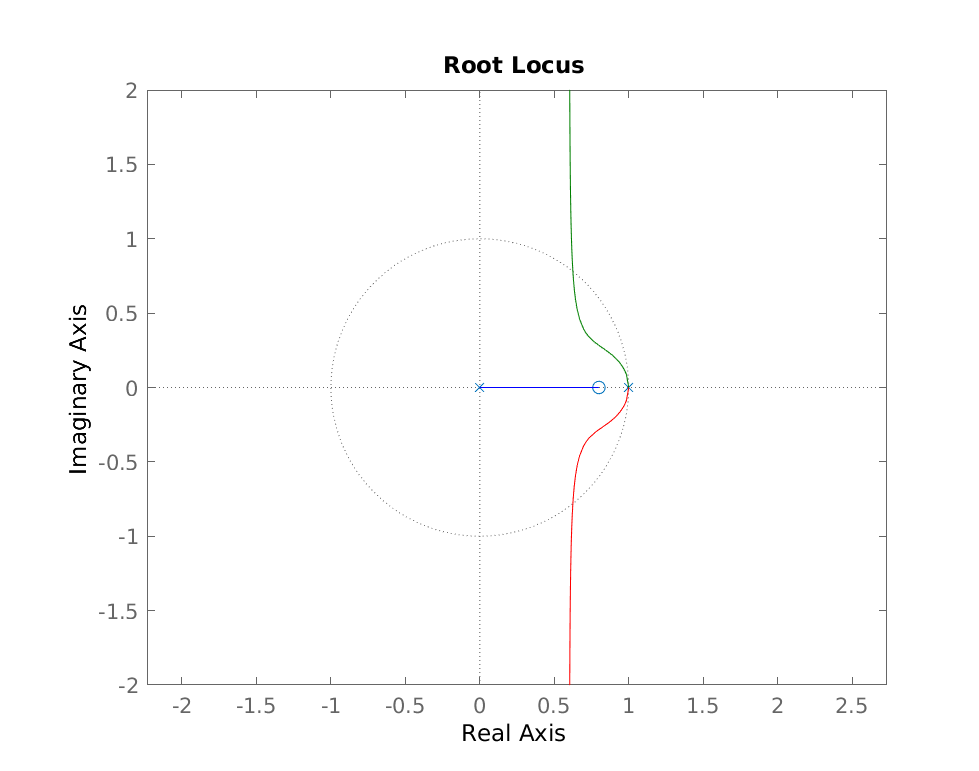
\includegraphics[width=0.6\linewidth]{rlocus-disk-arm.discrete}
\end{center}
\end{frame}

\begin{frame}[label={sec:orgceba539}]{Algebra en diagramas de bloque}
\begin{center}
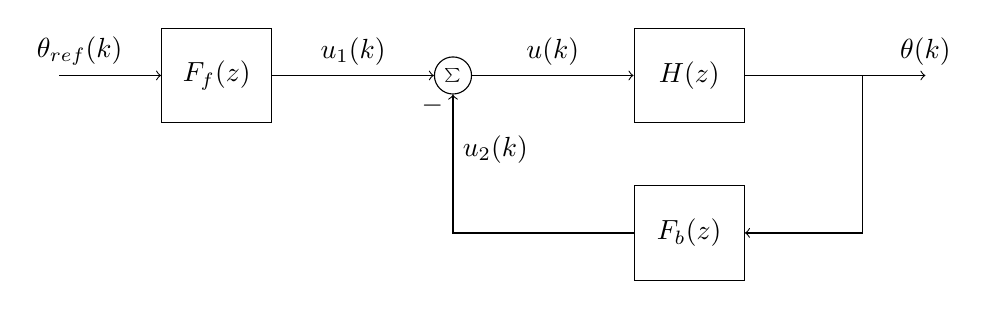
\begin{tikzpicture}
\tikzset{node distance=2cm, 
    block/.style={rectangle, draw, minimum height=12mm, minimum width=14mm},
    sumnode/.style={circle, draw, inner sep=2pt}        
}

  \node[coordinate] (input) {};
  \node[block, right of=input] (TR) {$F_f(z)$};
  \node[sumnode, right of=TR, node distance=30mm] (sum) {\tiny $\sum$};
  \node[block,right of=sum, node distance=30mm] (plant) {$H(z)$};
  %\node[sumnode, right of=plant, node distance=30mm] (sumdist) {$\sum$};
  %\node[coordinate, above of=sumdist, node distance=15mm] (dist) {};
  %\node[coordinate, right of=sumdist, node distance=15mm] (measure) {};
  \node[coordinate, right of=plant, node distance=30mm] (output) {};
  \node[coordinate, right of=plant, node distance=22mm] (measure) {};
  %\node[sumnode,below of=measure, node distance=25mm] (sumnoise) {$\sum$};
  %\node[coordinate, right of=sumnoise, node distance=15mm] (noise) {};
  \node[block,below of=plant, node distance=20mm] (SR) {$F_b(z)$};
  \draw[->] (input) -- node[above, pos=0.2] {$\theta_{ref}(k)$} (TR);
  \draw[->] (TR) -- node[above] {$u_1(k)$} (sum);
  \draw[->] (sum) -- node[above] {$u(k)$} (plant);
  \draw[->] (plant) -- node[at end, above] {$\theta(k)$} (output);
  \draw[->] (measure) |- (SR);
  \draw[->] (SR) -| (sum) node[right, pos=0.8] {$u_2(k)$} node[left, pos=0.96] {$-$};
\end{tikzpicture}
\end{center}
Usando \[U(z) = U_1(z) - U_2(z) = F_f(z)\Theta_{ref}(z) - F_b(z)\Theta(z), \quad \text{y}\]
\[ \Theta(z) = H(z)U(z), \quad \text{obtenemos} \]
\[ \Theta(z) = \underbrace{\frac{F_f(z)H(z)}{1 + F_b(z)H(z)}}_{H_c{z}} \Theta_{ref}(z). \]
\end{frame}

\begin{frame}[label={sec:orgd9f732f}]{Algebra en diagramas de bloque - pasos en detalle}
Usando \[U(z) = U_1(z) - U_2(z) = F_f(z)\Theta_{ref}(z) - F_b(z)\Theta(z), \quad \text{y}\]
\[ \Theta(z) = H(z)U(z), \quad \text{obtenemos} \]
\[ \Theta(z) = H(z)U(z) = H(z)\left(F_f(z)\Theta_{ref}(z) - F_b(z)\Theta(z)\right)\]
Mueve todos los terminos con \(\Theta\) al lado izquierdo:
\[ \Theta(z) + H(z)F_b(z)\Theta(z) = H(z)F_f(z)\Theta_{ref}(z)\]
\[ \Theta(z)\big(1 + H(z)F_b(z)\big) = H(z)F_f(z)\Theta_{ref}(z)\]
\[ \Theta(z) = \frac{H(z)F_f(z)}{1 + H(z)F_b(z)}\Theta_{ref}(z)\]
\end{frame}

\begin{frame}[label={sec:org50f2953}]{Estabilidad del sistem an lazo cerrado}
\[ \Theta(z) = \underbrace{\frac{F_f(z)H(z)}{1 + F_b(z)H(z)}}_{H_c{z}} \Theta_{ref}(z). \]

\begin{tcolorbox}
Estabilidad requiere que todos los polos del sistema, es decir las soluciones de la ecuación característica
\[ 1 + F_b(z)H(z) = 0\]
están en el interior del circulo unitario  del plano $z$.
\end{tcolorbox}
\end{frame}

\begin{frame}[label={sec:org6ba5318}]{Ejercicio}
\begin{center}
\begin{tikzpicture}
\tikzset{node distance=2cm, 
    block/.style={rectangle, draw, minimum height=12mm, minimum width=14mm},
    sumnode/.style={circle, draw, inner sep=2pt}        
}

  \node[coordinate] (input) {};
  \node[sumnode, right of=input, node distance=30mm] (sum) {\tiny $\sum$};
  \node[block, above of=sum] (TR) {$F_f(z)$};
  \node[block,right of=sum, node distance=20mm] (SR) {$F_e(z)$};
  \node[sumnode, right of=SR, node distance=20mm] (sum2) {\tiny $\sum$};
  \node[block,right of=sum2, node distance=30mm] (plant) {$H(z)$};
  %\node[sumnode, right of=plant, node distance=30mm] (sumdist) {$\sum$};
  %\node[coordinate, above of=sumdist, node distance=15mm] (dist) {};
  %\node[coordinate, right of=sumdist, node distance=15mm] (measure) {};
  \node[coordinate, right of=plant, node distance=30mm] (output) {};
  \node[coordinate, right of=plant, node distance=22mm] (measure) {};
  %\node[sumnode,below of=measure, node distance=25mm] (sumnoise) {$\sum$};
  %\node[coordinate, right of=sumnoise, node distance=15mm] (noise) {};
  \draw[->] (input) -- node[above, pos=0.2] {$\theta_{ref}(k)$} node[coordinate] (copy) {} (sum);
  \draw[->] (copy) |- (TR);
  \draw[->] (TR) -| node[above] {$u_1(k)$} (sum2);
  \draw[->] (sum) -- node[above] {$e(k) $} (SR);
  \draw[->] (SR) -- node[above] {$ u_2(k) $} (sum2);
  \draw[->] (sum2) -- node[above] {$u(k)$} (plant);
  \draw[->] (plant) -- node[at end, above] {$\theta(k)$} (output);
  \draw[->] (measure) -- ++(0,-20mm) -| (sum) node[left, pos=0.96] {$-$};
\end{tikzpicture}
\end{center}

\alert{Obtener la función de transferencia del lazo cerrado}
\end{frame}

\begin{frame}[label={sec:orgfa55875}]{Solución}
\[ U(z) = F_f(z)\Theta_{ref}(z) + F_e(z)E(z) = F_f(z)\Theta_{ref}(z) + F_e(z)\big(\Theta_{ref}(z) - \Theta(z)\big), \]
\[ \Theta(z) = H(z)U(z)\]
Entonces
   \begin{align*}
   \Theta(z) &= H(z)U(z) = H(z)\left(F_f(z)\Theta_{ref}(z) + F_e(z)\big(\Theta_{ref}(z) - \Theta(z)\big)\right)\\
 &= H(z)F_f(z)\Theta_{ref}(z) + H(z)F_e(z)\Theta_{ref}(z) - H(z)F_e(z)\Theta(z)\\
\big(1 + H(z)F_e(z)\big) \Theta(z) &= H(z)\big(F_f(z) + F_e(z)\big)\Theta_{ref}(z)\\
\Theta(z) &= \frac{H(z)\big(F_f(z) + F_e(z)\big)}{1 + H(z)F_e(z)}\Theta_{ref}(z)
\end{align*}
\end{frame}

\section{Estabilidad para el control del brazo del disko duro}
\label{sec:org9898629}

\begin{frame}[label={sec:org7eaa8f2}]{Estabilidad para el control del brazo del disko duro}
\begin{center}
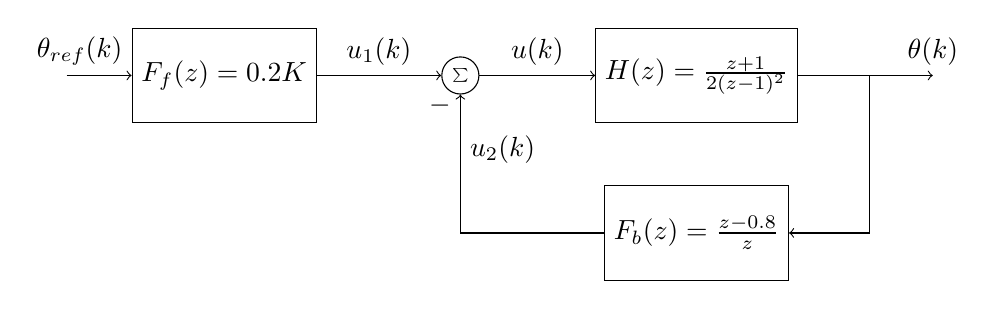
\begin{tikzpicture}
\tikzset{node distance=2cm, 
    block/.style={rectangle, draw, minimum height=12mm, minimum width=14mm},
    sumnode/.style={circle, draw, inner sep=2pt}        
}

  \node[coordinate] (input) {};
  \node[block, right of=input] (TR) {$F_f(z) = 0.2K$};
  \node[sumnode, right of=TR, node distance=30mm] (sum) {\tiny $\sum$};
  \node[block,right of=sum, node distance=30mm] (plant) {$H(z) = \frac{z+1}{2(z-1)^2}$};
  %\node[sumnode, right of=plant, node distance=30mm] (sumdist) {$\sum$};
  %\node[coordinate, above of=sumdist, node distance=15mm] (dist) {};
  %\node[coordinate, right of=sumdist, node distance=15mm] (measure) {};
  \node[coordinate, right of=plant, node distance=30mm] (output) {};
  \node[coordinate, right of=plant, node distance=22mm] (measure) {};
  %\node[sumnode,below of=measure, node distance=25mm] (sumnoise) {$\sum$};
  %\node[coordinate, right of=sumnoise, node distance=15mm] (noise) {};
  \node[block,below of=plant, node distance=20mm] (SR) {$F_b(z)=\frac{z-0.8}{z}$};
  \draw[->] (input) -- node[above, pos=0.2] {$\theta_{ref}(k)$} (TR);
  \draw[->] (TR) -- node[above] {$u_1(k)$} (sum);
  \draw[->] (sum) -- node[above] {$u(k)$} (plant);
  \draw[->] (plant) -- node[at end, above] {$\theta(k)$} (output);
  \draw[->] (measure) |- (SR);
  \draw[->] (SR) -| (sum) node[right, pos=0.8] {$u_2(k)$} node[left, pos=0.96] {$-$};
\end{tikzpicture}
\end{center}

\alert{Ecuación característica}
\begin{align*}
1 + H(z)F_b(z) &= 0\\
1 + \frac{z+1}{2(z-1)^2}K\frac{z-0.8}{z} &= 0\\
(z-1)^2z + \frac{K}{2}(z+1)(z-0.8) &= 0
\end{align*}
\end{frame}


\begin{frame}[label={sec:org6884b60}]{Estabilidad para el control del brazo del disko duro}
\alert{Actividad en grupo} Completar el diagrama de lugares de los raíces abajo
\[(z-1)^2z + \frac{K}{2}(z+1)(z-0.8) = 0\]
\begin{center}
  \begin{tikzpicture}[scale=2.5]
    \draw[->] (-1.2, 0) -- (1.2,0);
    \draw[->] (0, -1.2) -- (0,1.2);
    \node[red, pin=45:{2 polos del proceso}] at (1,0) {\large $\times$};
    \node[red, pin=135:{polo del controlador}] at (0,0) {\large $\times$};
    \node[green!70!black, pin=-145:{cero de controlador}] at (0.8,0) {\Large $\circ$};
    \node[green!70!black, pin=-145:{cero del proceso}] at (-1,0) {\Large $\circ$};
    \node at (0.8, -0.2) {$0.8$};
    \node at (1, -0.2) {$1$};
    \draw[domain=0:360, samples=361, dashed] plot ({cos(\x)}, {sin(\x)});
    \node[coordinate, pin=60:{$|z|=1$}] at (0.5, 0.87) {};
  \end{tikzpicture}
\end{center}
\end{frame}
\end{document}